\subsection{MobileNet}
\begin{frame}{}
    \LARGE CNN Architectures: \textbf{MobileNet}
\end{frame}

% MobileNet
\begin{frame}{Motivation for MobileNets}
    \begin{itemize}
        \item \textbf{Why MobileNets?}
        \begin{itemize}
            \item Small-sized models are crucial for mobile and embedded devices.
            \item MobileNets reduce computational cost and memory usage while maintaining good accuracy.
        \end{itemize}
        \item \textbf{Key Idea:}
        \begin{itemize}
            \item Use \textbf{depthwise-separable convolutions} to significantly reduce computation compared to standard convolutions.
        \end{itemize}
    \end{itemize}
\end{frame}

\begin{frame}{Computational Cost of Convolutions}
    \begin{itemize}
        \item \textbf{Computational cost of standard convolution:}
        \[
        \text{Cost} = \text{\# filter params} \times \text{\# filter positions} \times \text{\# filters}
        \]
        \item Filters operate on all input channels, increasing computation significantly.
    \end{itemize}
    \begin{figure}
        \centering
        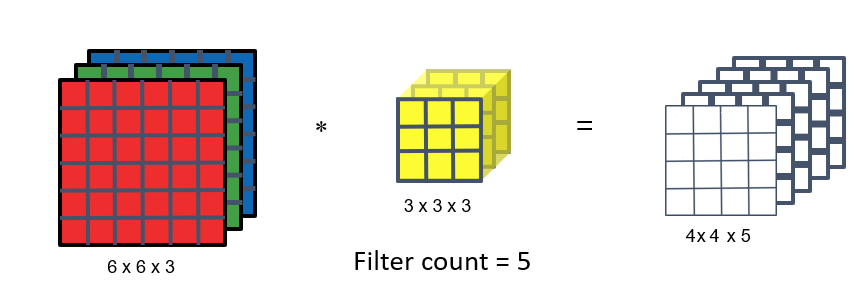
\includegraphics[width=0.8\linewidth]{images/cnn/NormalConv_MobileNet.png} 
    \end{figure}
\end{frame}

\begin{frame}{Depthwise-Separable Convolutions}
    \begin{itemize}
        \item Split standard convolution into two steps:
        \begin{itemize}
            \item \textbf{Depthwise Convolution:} Applies a single filter per input channel.
            \item \textbf{Pointwise Convolution:} Combines outputs from depthwise convolution.
        \end{itemize}
        \item \textbf{Key Benefit:} Reduces computational cost significantly compared to standard convolution.
    \end{itemize}
    \begin{figure}
        \centering
        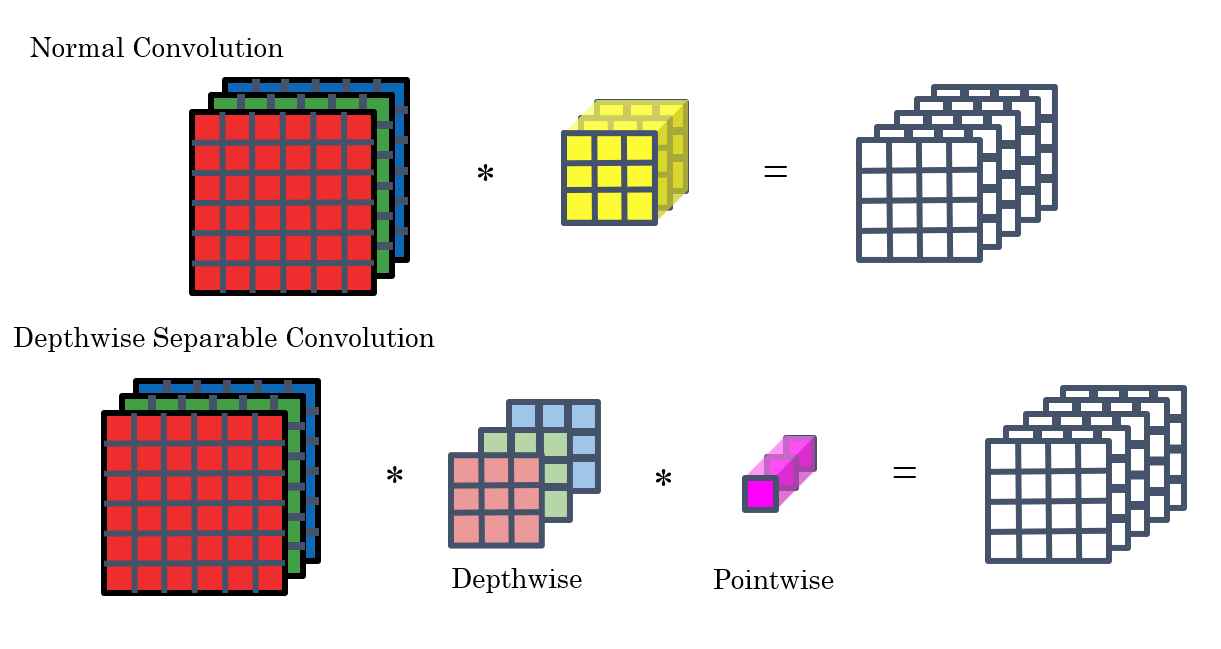
\includegraphics[width=0.8\linewidth]{images/cnn/Depth_vs_Normal_Conv.png} 
    \end{figure}
\end{frame}

\begin{frame}{Depthwise Convolution}
    \begin{itemize}
        \item Operates on each input channel separately.
    \end{itemize}
    \begin{figure}
        \centering
        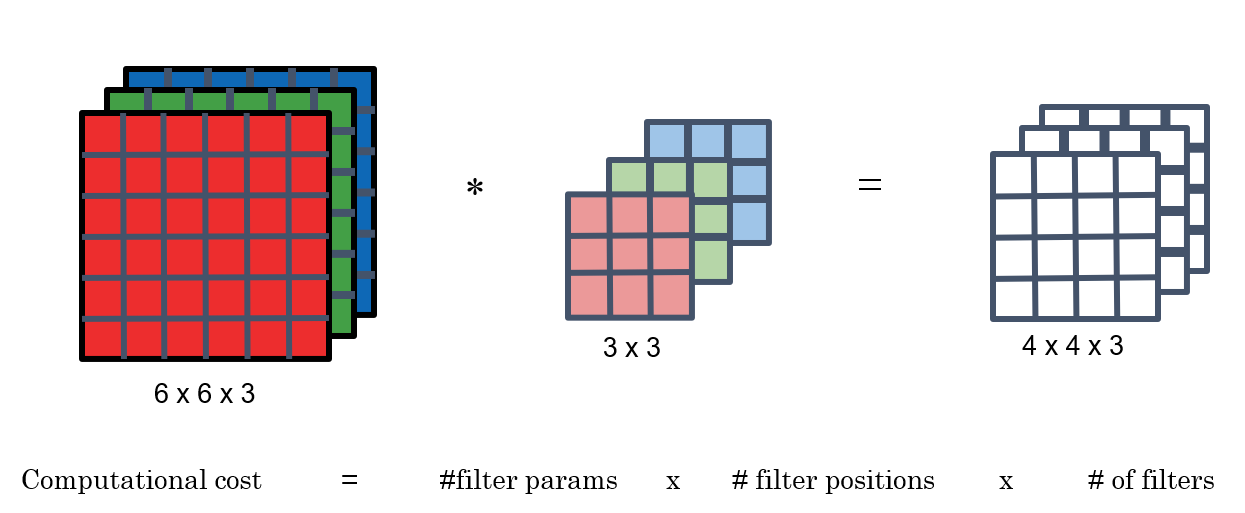
\includegraphics[width=0.8\linewidth]{images/cnn/Depthwise_conv.png}
    \end{figure}
\end{frame}


\begin{frame}{Pointwise Convolution}
    \begin{itemize}
        \item Combines outputs from depthwise convolution using \(1 \times 1\) convolutions (mixes channels).
    \end{itemize}
    \begin{figure}
        \centering
        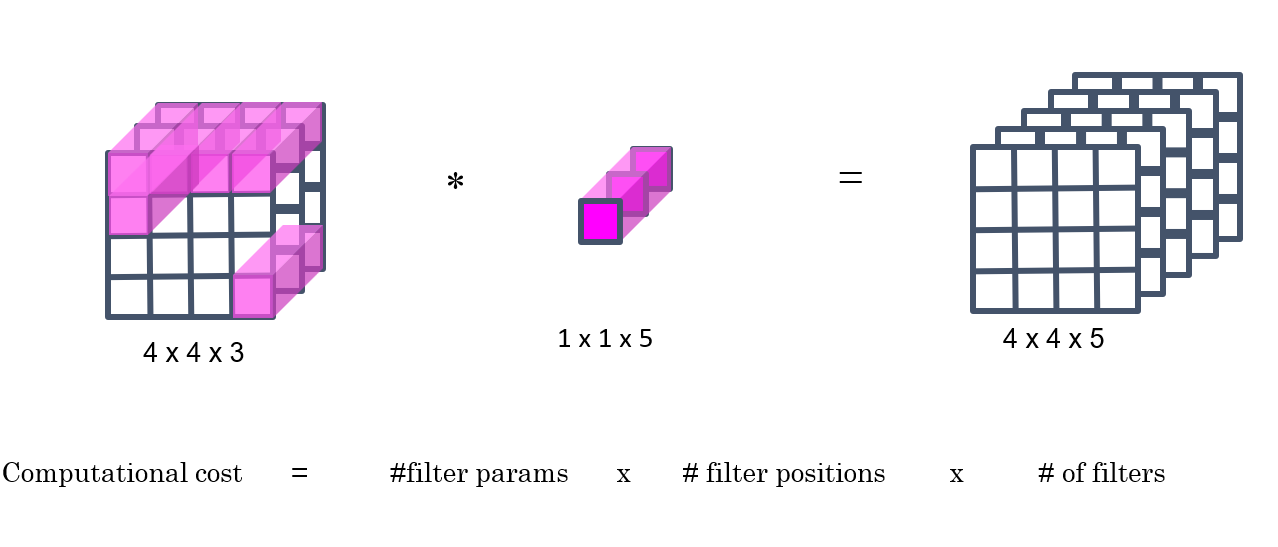
\includegraphics[width=0.8\linewidth]{images/cnn/PointWise_conv.png}
    \end{figure}
\end{frame}

\begin{frame}{MobileNet Architectures}
    \begin{itemize}
        \item \textbf{MobileNet v2:}
        \begin{itemize}
            \item Adds \textbf{residual connections}.
            \item Introduces:
            \begin{itemize}
                \item \textbf{Expansion step:} Expands input dimensions before depthwise convolution.
                \item \textbf{Projection step:} Reduces dimensions after processing.
            \end{itemize}
        \end{itemize}
    \end{itemize}
    \begin{figure}
        \centering
        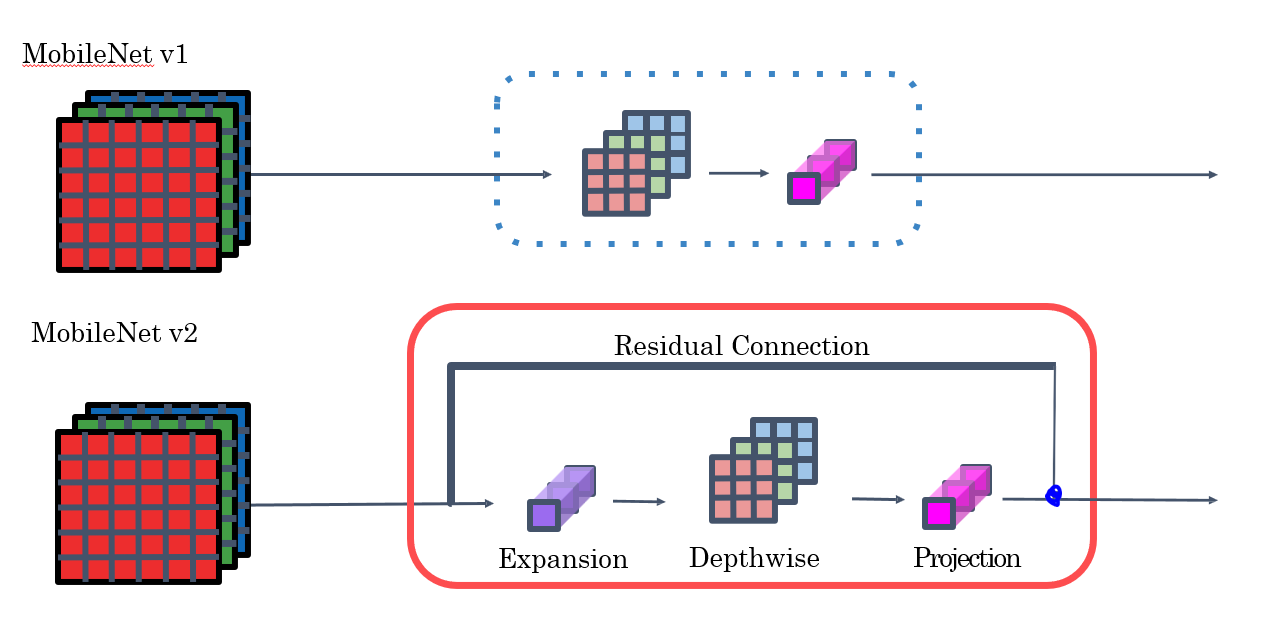
\includegraphics[width=0.8\textwidth,height=.7\textheight,keepaspectratio]{images/cnn/MobileNet_1_and_2.png} 
    \end{figure}
\end{frame}